\chapter{Triggering in the di-$b$-jet analysis}
\label{sec:trig}

As described in Section~\ref{sec:det-trig},
ATLAS does not have the resources to process or store all the data from the 40~MHz of collisions delivered by the LHC.
To solve this problem the ATLAS trigger system performs the vital role of
reducing the rate of data-taking to 1~kHz by selecting events containing a high-$p_T$ object.\\

As a result all analyses must chose a trigger strategy and understand the impact of this trigger on their analysis.
In the di-$b$-jet analysis we use a single jet trigger for the high-mass channel
and a double $b$-jet trigger for the low-mass channel.
This chapter aims to provide a detailed description of the triggers used in this analysis,
and as such is organised in the following manner;
Section~\ref{sec:trig-jet} provides a brief description of jet triggers as used in the high-mass channel and the limitations of this approach,
Section~\ref{sec:trig-bjet} contains a description of $b$-jet triggers that are used in the low-mass channel
and finally Section~\ref{sec:trig-bjet_eff} presents the measurement of the $b$-jet trigger efficiency, an essential input of the low-mass channel.

\section{Jet-Triggers}
\label{sec:trig-jet}

Jet-triggers are tasked with selecting events with one or more jets from the deposits in the ATLAS calorimeter system,
this is one of most challenging triggers in any hadron-hadron collider due to extremely high cross-sections of hadronic jet production~\cite{trig-run2_proc}.
In Run-2 the jet-triggers are used at both L1 and HLT level; each using different levels of information and different algorithms,
so are described separately within this section.


\subsection{Level 1}

The L1 trigger is a hardware based trigger which accepts or rejects an event within \SI{2.2}{\micro\second}.
The L1 jet-trigger receives trigger towers from the calorimeter;
where a trigger tower is the measured energy deposit in a cell of the ECAL or HCAL of granularity 0.1x0.1 in the $\eta-\phi$ plane.
In the L1 trigger hadronic jet algorithms search for a neighbouring group of 4x4 trigger towers containing energy deposits above some pre-set threshold.
Our analysis uses the L1 trigger known as \verb|L1_J100|, which requires that at least one trigger tower group with an energy deposit of \SI{100}{\GeV} has been found.
Other L1 triggers that search for multiple clusters are also possible to reduce the energy thresholds required.
The L1 trigger can then seed the HLT trigger.
It is also worth noting that at L1 there is no tracking information, meaning that electron and taus
are also triggered on using similar techniques as hadronic jet algorithms, except using narrower groups of trigger towers.
\\

\subsection{HLT}

The HLT trigger is a software based trigger which, due to the lower input rate and larger time window,
is able to use more complex algorithms to reconstruct jets.
At the HLT level jets are reconstructed using topoclusters (TCs) constructed from neighbouring cells selected using the cell's energy significance ($E/\sigma$);
TCs are seeded from cells with $E/\sigma > 4$, then neighbouring cells with $E/\sigma > 2$ are added
and finally all neighbouring cells around are also added.
Jets are then reconstructed from the topoclusters;
in this analysis we use jets that have been reconstructed using
the anti-$k_T$ algorithm with an $R = 0.4$ \footnote{Section~\ref{sec:obj-jets} \textit{(sec:obj-jets)} defines these terms}.

\subsection{High-mass trigger selection}

For the high-mass analysis we use the trigger \verb|HLT_j380|, that is fired when a jet is found with a $p_T >$ 380 GeV.
This is chosen as it is the lowest un-prescaled single jet-trigger;
meaning that of triggers that accept every event passing a single jet criteria,
this trigger has the lowest jet-$p_T$ threshold.
Due to the exponential increase in jet production cross-section at low jet-$p_T$,
the $p_T$ threshold is set to keep the acceptance rates low enough such that the HLT trigger is within its output rate budget of 1~kHz.\\

However, as will be discussed further in Section~\ref{sec:evtSel}\textit{(sec:evtSel)},
this $p_T$ threshold limits the high-mass di-$b$-jet analysis to only select events with $m_{jj} >$ 1.2~TeV,
otherwise the $m_{jj}$ range will enter a kinematic region where
trigger acceptance is less than 1 in such a way that the QCD background is sculpted
in a manner that the background modelling can not adapt to.
To reach to lower masses a different trigger strategy is required.\\

\section{$b$-Jet Triggers}
\label{sec:trig-bjet}

In this analysis we search for pairs of $b$-jets,
which, as described in Section~\ref{sec:obj-bjets}\textit{(sec:obj-bjets)},
can be identified from the topology of tracks in the inner detector indicating that a $B$-hadron was within the jet.
This additional selection at the trigger level reduces rates significantly
\footnote{It is known that the QCD background is dominated by light-jets, see Figure~\ref{fig-dibjet_backgroundFlav}\textit{Plot of background flav comp}}
allowing a lower jet-$p_T$ threshold than was used by the single jet-$p_T$ trigger, and hence lower $m_{jj}$ values to be accessed.
$b$-jet triggers have been used in a range of previous ATLAS analyses,
including for HH to 4 $b$-jets~\cite{trig-H4b}.\\

\subsection{General description}

In 2016 data, the $b$-jet trigger configuration contains three steps~\cite{trig-bTrig_desc},
making use of the regions of interest (RoI) described by the jets found by the jet-trigger.
Firstly, a `fast'-tracking algorithm is run in a super-RoI
which is formed around all jets in the event which have $E_T >$ 30 GeV;
these tracks are then used to identify the primary vertex in the event.
Secondly, within each jet RoI precision tracking is run, with a constraint on the PV position from the first step.
Finally, these tracks are the input to the multi-variate $b$-tagging algorithm described in
Section~\ref{sec:obj-bjets_MV2}\textit{(sec:obj-bjets\_MV2)} to identify $b$-jets.
There are several $b$-jet triggers available in the ATLAS trigger menu;
with a variety of requirements on the jet multiplicity, number of tagged jets and $b$-tag operating point used.
Figure~\ref{fig:trig-bTrig_perf} shows ROC curves representing the expected performance of Run-2 $b$-trigger.
\\

\begin{figure}[!ht]
  \begin{center}
    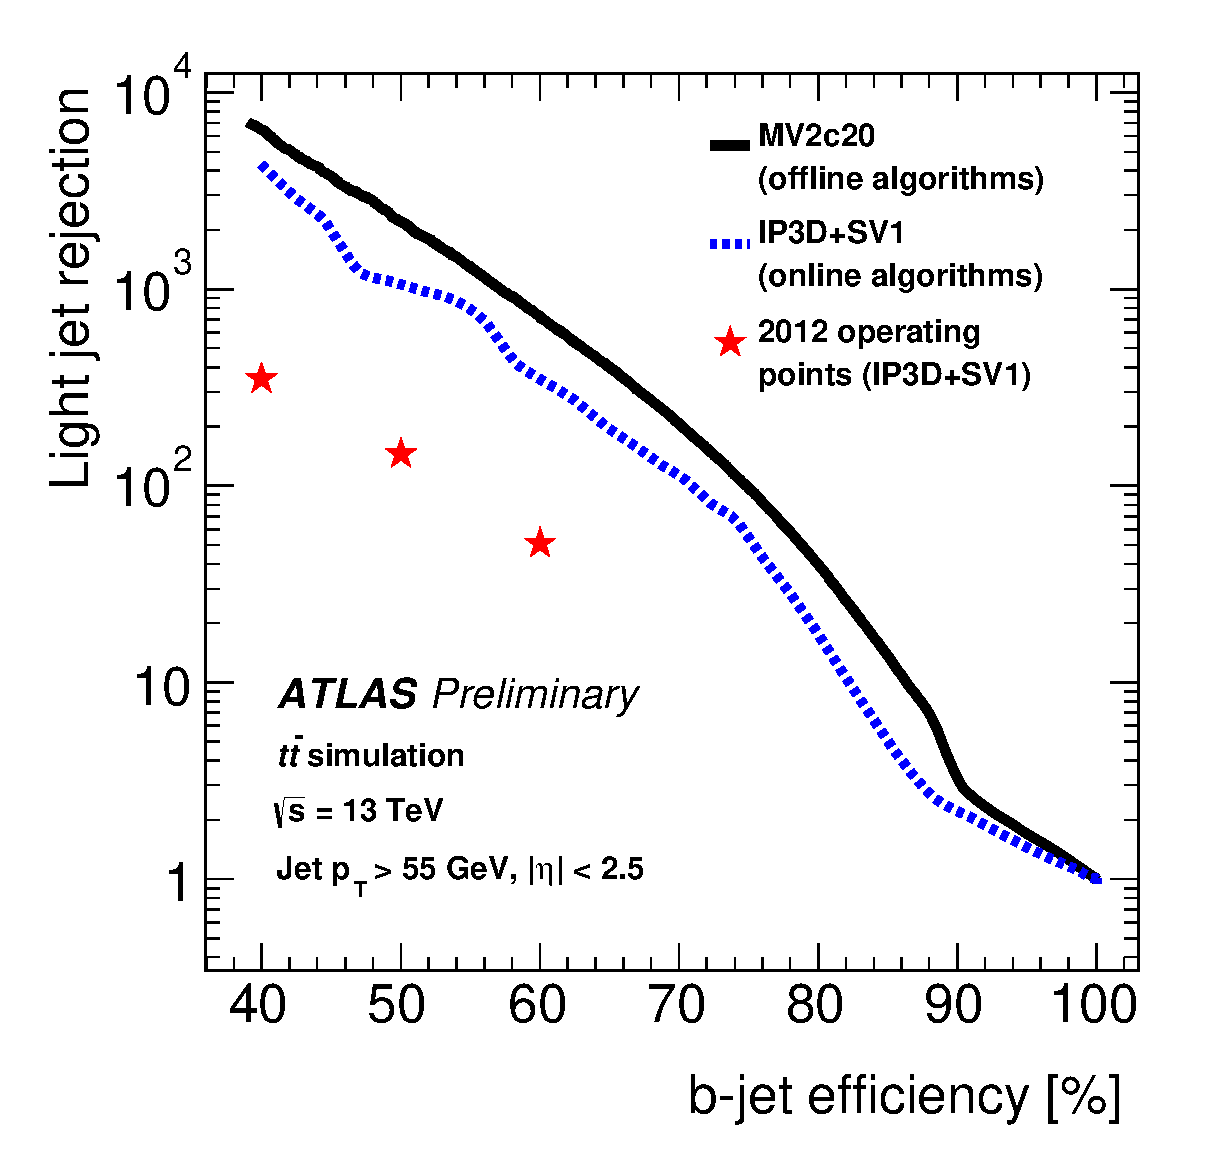
\includegraphics[width=0.48\linewidth, angle=0]{figs/Trigger/trig-bTrig_perf_light.eps}
    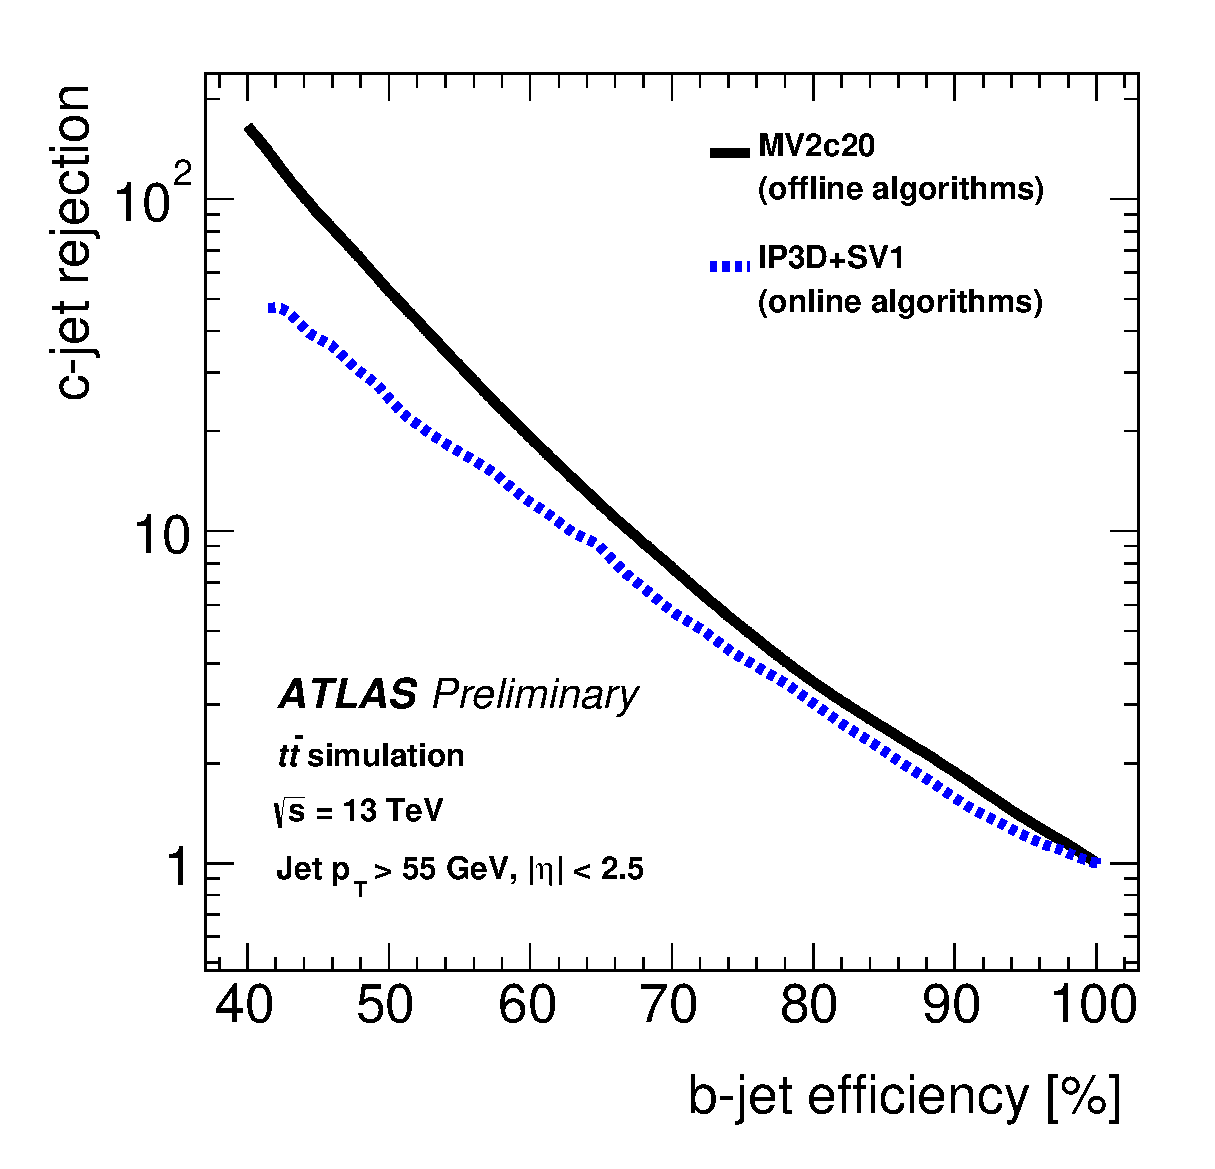
\includegraphics[width=0.48\linewidth, angle=0]{figs/Trigger/trig-bTrig_perf_charm.eps}
  \end{center}
  \caption{The expected $b$-jet efficiency of $b$-jet triggers with respect to (a) light-jet and (b) $c$-jet rejection
    in the case where the $b$-tagging algorithm used is MV2c20 (Black), IP3D+SV1 (Blue) and for the set-up used in Run-1 (red stars).}
  \label{fig:trig-bTrig_perf}
\end{figure}

There are few subtleties worth commenting on the $b$-jet trigger configuration, which affect decisions taken in this analysis.
One is that on this figure we see two lines corresponding to different $b$-tagging algorithms used in $b$-jet trigger;
IP3D+SV1 was used in 2015 data-taking,
whilst the MV2c20 was used in 2016 data-taking.
Another difference between 2015 and 2016 is the primary vertex finding algorithm used;
2016 data-taking employed a more complicated algorithm based on what is used offline, know as \textit{xPrmVtx},
whilst in 2015 an algorithm using a simple histogram based approach was employed, known as \textit{EFHist}. \\

Finally it is worth noting that there are  differences between online and offline $b$-tagging that will have an impact on what is to follow.
Firstly, coarser tracking information is available online, notably online tracks are not reconstructed from the whole range of the detector.
Secondly, a slightly different training setup is used for the multi-variate algorithm, mainly that a different fraction of $c$-jets were present in the training sample
(10\% offline vs. 20\% online).\\

In this analysis we use the double $b$-jet trigger,
\begin{center}
\verb|HLT_j150_bmc2c2060_split_j50_bmv2c2060_split|
\end{center}
which triggers on two jets with $p_T >$ 150 and 50 GeV respectively,
which have been $b$-tagged at the 60\% efficiency working point.\\

\section{Efficiency Measurement of the $b$-Jet Trigger}
\label{sec:trig-bjet_eff}

Any part of the ATLAS detector framework needs to be understood and calibrated with data for use in an analysis;
and this includes the trigger which can have a large impact on the analysis.
In this section I discuss the strategy and results of the $b$-jet trigger measurement in 2016,
which is an important input to the low-mass channel of the di-$b$-jet analysis.
\\

\subsection{Strategy}
The $b$-jet trigger is always used in tandem with offline $b$-tagging which is calibrated independently of the $b$-trigger.
Hence, to do this measurement whilst making use of the offline $b$-tagging calibrations already available,
we measure the $b$-jet trigger efficiency with respect to offline $b$-tagging, $\epsilon_{bTrig}$,
which is defined as the number of offline-tagged true $b$-jets that match an online-tagged trigger-jet by the number of offline tagged $b$-jets that match a trigger jet.
Or to put this in an equation;
\begin{equation}
 \epsilon_{bTrig} = \frac{N(\text{Offline-tagged, online-tagged, true $b$-jets)}}{N(\text{Offline-tagged, trigger-matched, true $b$-jets)}}
\end{equation}
This quantity can be interpreted as the probability that a true $b$-jet is tagged at the trigger-level,
given that it there is a jet at the trigger level and that it would be $b$-tagged at the offline stage.

To measure $\epsilon_{bTrig}$ we require a sample that has high $b$-jet purity,
such that we have confidence that the jets we use to calculate this ratio are true $b$-jets.
We also need to be able to trigger on this sample in such a way that we are not biasing ourselves from using $b$-tagging online;
or simply put we cannot use the $b$-jet trigger to select events.
The sample we use to fill these criteria is a di-lepton $t\bar{t}$ sample containing a muon and an electron.
Top-quarks decay to a $W$-boson and a $b$-quark with almost 100\% branching ratio meaning that this sample provides a good source of $b$-quarks,
but also the electron and muon give a distinct signature which allows us to select this process with good purity and gives a non-$b$-jet object to trigger on.
The exact event selection is described below. \\

The $b$-jet trigger efficiency is determined in data and is compared to the efficiency found in a 
simulated $t\bar{t}$ sample which is used to extrapolate the efficiency to 
higher jet-$p_T$ where the data-derived efficiency loses statistical precision.
The efficiency in data, including the simulation based extrapolation, can then be
compared to simulation to derive a Data/Monte-Carlo scale factor, which is used as the input to the analysis.
\\

$\epsilon_{bTrig}$ and Data/Monte-Carlo scale factors are derived for all combinations of offline and online $b$-tagging working points.
However, we will show the process for the 70\% offline and 60\% online working point
as this is set of working points used in this analysis.

\subsection{Datasets}
The data used for this analysis is the full 2016 ATLAS data-set.
In addition to the usual data-quality requirements applied,
as discussed in Section~\ref{sec:evtSel_GRL}\textit{(sec:evtSel\_GRL)},
a $b$-jet trigger aware Good Run List (GRL)
\footnote{A GRL is effectively a list of lumi-blocks that pass certain data-quality requirements.
  As mentioned in the text a further discussion is held here in Section~\ref{sec:evtSel_GRL}\textit{(sec:evtSel\_GRL)}}
applies the requirement that the online beamspot is within 2mm of the origin in Periods A-I of the data.
This means that the data-set contains 24.5~\ifb of data.
A discussion of the requirement for this GRL is in Section~\ref{sec:trig-inv}. \\

For the simulated $t\bar{t}$ sample, the generation is performed with
a Powheg-Box v2~\cite{trig-powheg} generator with the CT10 PDF sets in the matrix element calculations is used.
We will also consider a simulated single-top sample;
electroweak t-channel, s-channel and $Wt$-channel single top-quark events are generated using the Powheg-Box v1 generator.
This generator uses the 4-flavour scheme for the NLO matrix elements calculations together with the fixed four-flavour PDF set CT10f4.
%For all top processes, top-quark spin correlations are preserved (for t-channel, top quarks are decayed using MadSpin[10a]).
The parton shower, fragmentation, and the underlying event are simulated using Pythia6.428~\cite{trig-pythia6} with the CTEQ6L1~\cite{trig-CTEQ6L1} PDF sets
and the corresponding Perugia 2012 tune (P2012)~\cite{trig-perugia}.
The top mass is set to 172.5 GeV.
The EvtGen v1.2.0 program~\cite{trig-evtGen} is used for properties of the bottom and charm hadron decays. \\

\subsection{Event Selection}

A high-purity sample of $b$-jets is selected using a di-lepton $t\bar{t}$ selection.

\noindent
The event selection is summarised as follows:

\begin{itemize}
\item The event fired a single lepton bperf trigger which are:
    \begin{itemize}[label={$-$}]
      \item\verb|HLT_mu26_imedium_2j35_bperf|
      \item\verb|HLT_e26_tight_iloose_2j35_bperf|
      \item\verb|HLT_e26_lhtight_iloose_2j35_bperf|
    \end{itemize}
\item At least 1 medium muon: $\pT>25~\GeV$, which has no jet within a $\Delta R$ of 0.4.
\item At least 1 medium electron: $\pT>25~\GeV$.
\item 2 offline $b$-tagged jets:
   \begin{itemize}[label={$-$}]
     \item Offline R=0.4 anti-$k_T$ jets.
     \item $\pT>35~\GeV$ and $|\eta|<2.5$.
     \item Offline $b$-tagged at the 85\%~operating point.
     \item Jet must be matched to a trigger-jet.
    \end{itemize}
\end{itemize}
\vspace{1em}

Descriptions of the object-definitions of muons, electrons, jets and $b$-tagged can be found in
Sections~\ref{sec:object_muon}\textit{(sec:object\_muon)},~\ref{sec:object_electron}\textit{(sec:object\_elec)},~\ref{sec:object_jet}\textit{(sec:object\_jet)}
and \ref{sec:object_bjet}\textit{(sec:object\_bjet)} respectively.
Online trigger jets are matched to offline jets using $\Delta R$ matching, requiring for a match the jets must have $\Delta R<0.6$.\\

The triggers used are bperf trigger, which are special triggers used in data-taking specifically for monitoring the $b$-jet trigger performance.
They fire if a muon or an electron with $\pT > 26 GeV$ is reconstructed at the trigger level.
The bperf triggers then run the online $b$-tagging algorithm on all trigger jets with $|\eta|<2.5$ and
$p_{T}>35~GeV$ without performing any cuts on the output of the multi-variate algorithm; ensuring there is no bias in the efficiency measurement. \\

\subsection{The Initial Problem}

To give context to the following section;
the first discussion will be what was first observed when measuring the $b$-jet efficiency.
Figure~\ref{fig:trig-Full_noGRL_eff_noHLTMatch} shows $\epsilon_{b-Trig}$,
when no $b$-jet trigger aware GRL is not applied
and no requirement on offline jets matching a trigger jet is required in the denominator.
In addition we can see that there is a clear shape in the jet-$\eta$ distributions that needs to be understood.
This shows the efficiency in data is substationally below the efficiency expected from simulation,
an effect that needs to be investigated and understood properly.

\begin{figure}[!ht]
  \begin{center}
    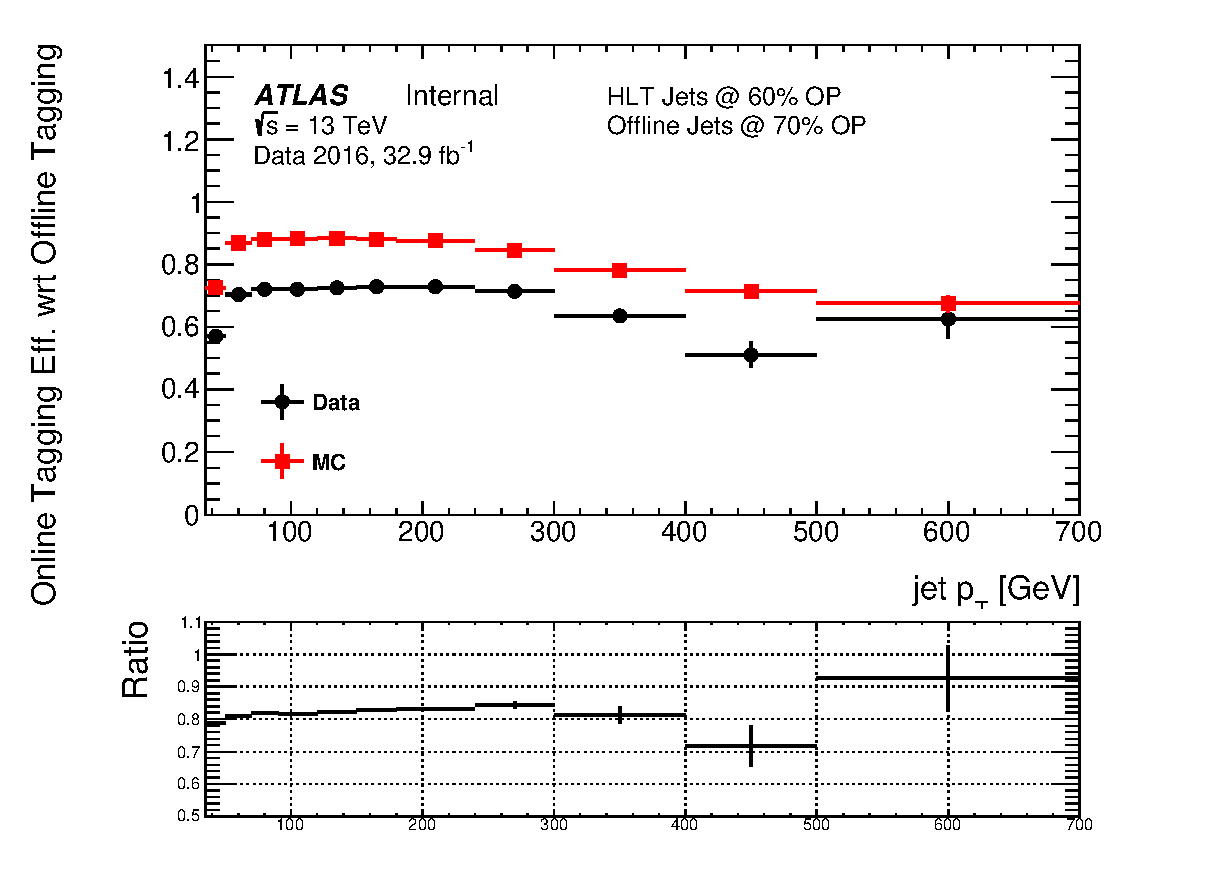
\includegraphics[width=0.48\linewidth, angle=0]{figs/trigger/Full_noGRL_eff_noHLTMatch_jetPt.eps}
    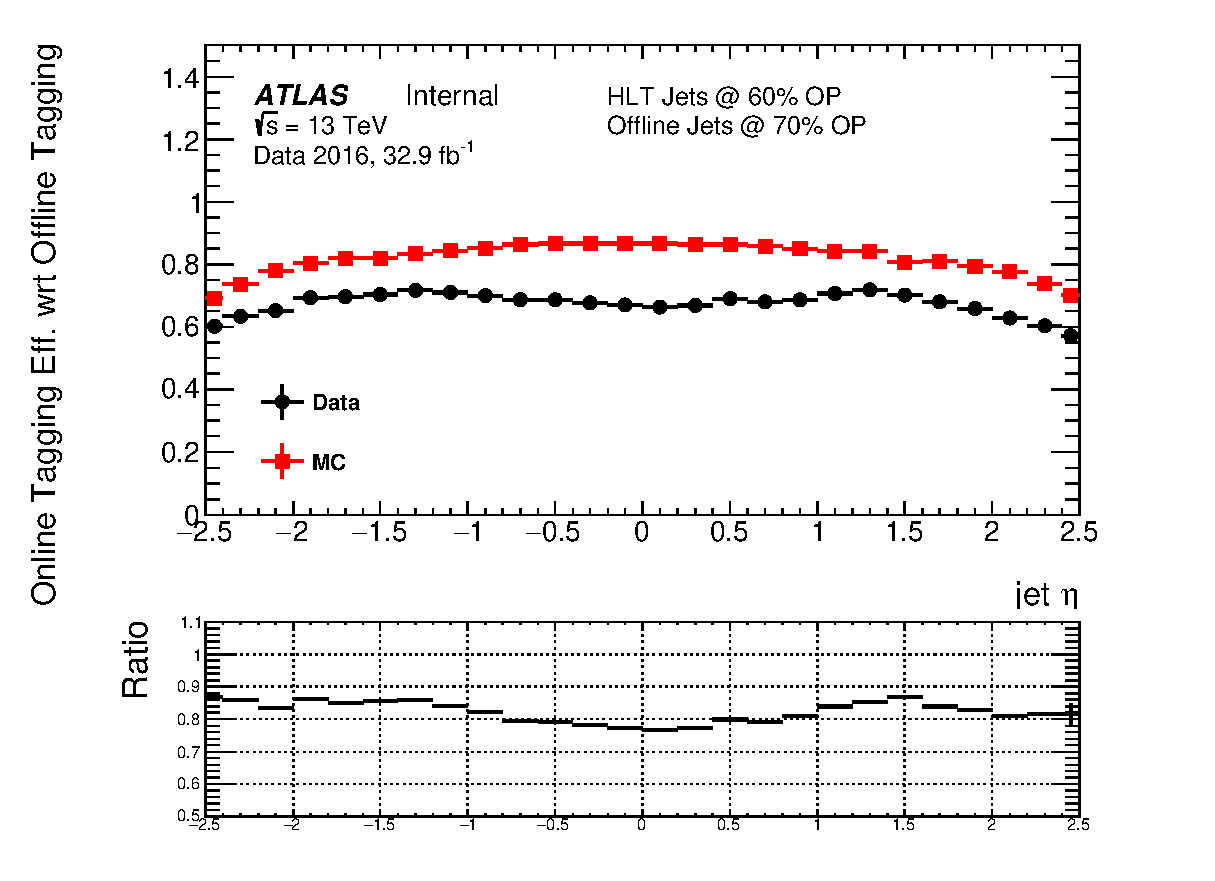
\includegraphics[width=0.48\linewidth, angle=0]{figs/trigger/Full_noGRL_eff_noHLTMatch_jetEta.eps}
  \end{center}
  \caption{The 60\% $b$-jet trigger efficiency with respect to an offline 70\% operating point tag
    for data from Data (black) and simulation (red) against jet-\pT~(left), jet-$\eta$ (right).
    The $b$-trigger aware GRL is not applied and trigger matching is not required.}
  \label{fig:trig-Full_noGRL_eff_noHLTMatch}
\end{figure}

\subsection{Investigation and Solution}
\label{sec:trig-inv}

Given the disagreements between data and simulation we performed a number of cross-checks to understand this discrepancy,
including period dependance, detector performance, pile-up conditions and onlin beamspot position peformance.
In this section,
I summarise the results of the investigation
and demonstrate the $b$-trigger performance in 2016 data. \\

As described above, in 2016 data an algorithm known as \textit{xPrmVtx} was used.
It has since been uncovered that there was a bug in the code used to implament this algorithm;
effectively different co-ordinates were used by components of the code.
Online tracks passed to \textit{xPrmVx} use position with repect to online beam-spot position,
where the \textit{xPrmVx} algorithm assumed track position with respect to the origin.
This means that when the online beam-spot $z$-position is far from from the origin,
a vertex with position at the origin is passed to the $b$-tagging algorithms,
which leads to sub-optimal performance.
This will be shown below.

The exact setup for the $b$-jet trigger has changed as data has taken, to respond to performance issues as they are noticed and patches are applied
As such the relevant conditions of the $b$-jet trigger can be split into three regions of data-taking, which I will refer to as epochs,
and the effect of \verb|xPrmVx| returning a dummy vertex on $b$-jet trigger performance is different in each of these epochs.
Table~\ref{tab:bJetTrigEpochs} summaries the effect on the $b$-jet trigger of not finding a valid xPrmVtx vertex on the $b$-jet trigger in each epoch.
As a result of these differences in trigger performance, each epoch is now considered studied independantly. \\
\begin{table}[!htb]
  \begin{tabular}{ | c || c | c | l |}
    \hline			
    Epoch & Runs & Periods & Effect if no xPrmVtx PV is found \\ \hline
    1 & \parbox[t]{2.5cm} {296939-300571, \\ 300655}  & A,B(part)             & \parbox[t]{5cm} {An invalid vertex is used by the online b-tagging resulting in very low $\epsilon_{bTrig}$} \\
    \hline
    2 & \parbox[t]{2.5cm} {300600, \\ 300784-308084\\}  & B(part),C,D,E,F,G,I,J & \parbox[t]{5cm} {The b-jet trigger is not fired\\ } \\
    \hline
    3 & \parbox[t]{2.5cm} {309331-311481\\}       & K,L                     & \parbox[t]{5cm} {A back-up primary vertex \\ finding algorithm is used.} \\
    \hline
  \end{tabular}
  \vspace{10pt}
  \caption{A table describing the effect of not finding a valid xPrmVtx primary vertex on different epochs of data.}
  \label{tab:trig-epochs}
\end{table}

%For Epoch 1, the $\epsilon_{bPerf}$ is 100\% as shown in Figure~\ref{fig:Epoch1_bperf} for Period A.
In Epoch 1, due to the use of an invalid vertex, as described in Table~\ref{tab:bJetTrigEpochs},
there is a lower  $\epsilon_{bTrig}$ compared to that measured in simulation,
as shown in Figure~\ref{fig:Epoch1_eff} for Epoch 1.
The variable vertex class, shown in Figure~\ref{fig:Epoch1_eff}, is defined as 0 when a valid xPrmVtx vertex is found and 1 if not.


%\begin{figure}[!ht]
%\begin{center}
%  \includegraphics[width=0.45\linewidth, angle=0]{figs/Trigger/btrigger_old/Epoch1_trigReq_bPerfEff_jetPt.pdf}
%  \includegraphics[width=0.45\linewidth, angle=0]{figs/Trigger/btrigger_old/Epoch1_trigReq_bPerfEff_bs_online_vz.pdf}
%\end{center}
%\caption{$b$-perf efficiency, $\epsilon_{bPerf}$, for data from Period A (black) and simulation (red) against jet-pT~(left) and online beamspot z-position (right).}
%\label{fig:Epoch1_bperf}
%\end{figure}

\begin{figure}[!ht]
\begin{center}
  \includegraphics[width=0.45\linewidth, angle=0]{figs/Trigger/btrigger_old/Epoch1_trigReq_eff_jetPt.pdf}
  \includegraphics[width=0.45\linewidth, angle=0]{figs/Trigger/btrigger_old/Epoch1_trigReq_eff_jetEta.pdf} \\
  \includegraphics[width=0.45\linewidth, angle=0]{figs/Trigger/btrigger_old/Epoch1_trigReq_eff_vtxClass.pdf}
  \includegraphics[width=0.45\linewidth, angle=0]{figs/Trigger/btrigger_old/Epoch1_trigReq_eff_bs_online_vz.pdf}
\end{center}
\caption{The 60\% $b$-jet trigger efficiency with respect to an offline 70\% operating point tag
  for data from Epoch 1 (black) and simulation (red) against jet-\pT~(upper left),
  jet-$\eta$ (upper right), vertex class (lower left) and online beamspot z-position (lower right).}
\label{fig:Epoch1_eff}
\end{figure}

For Epoch 2, due to the b-jet trigger not firing when an xPrmVtx PV is not found, as described in Table~\ref{tab:bJetTrigEpochs},
we find that there are no online b-tagged jets for some events.
To account for this, in addition to $\epsilon_{bTrig}$, we must measure the b-perf efficiency, $\epsilon_{bPerf}$,
the efficiency that there are online jets in an event to match the offline jets.
$\epsilon_{bPerf}$ is calculated by dividing the number of events that pass the trigger
\verb|HLT_mu26_imedium_2j35_bperf| by the number that pass the trigger \verb|HLT_mu26_imedium|.
A lower $\epsilon_{bPerf}$ efficiency is observed in Epoch 2 than in simulation,
as shown in Figure~\ref{fig:Epoch2_eff}.
However in Epoch 2, $\epsilon_{bTrig}$ is measured to be in agreement with simulation within 5\%.

\begin{figure}[!ht]
\begin{center}
  \includegraphics[width=0.45\linewidth, angle=0]{figs/Trigger/btrigger_old/Epoch2_trigReq_bPerfEff_jetPt.pdf}
  \includegraphics[width=0.45\linewidth, angle=0]{figs/Trigger/btrigger_old/Epoch2_trigReq_bPerfEff_bs_online_vz.pdf}
\end{center}
\caption{$b$-perf efficiency, $\epsilon_{bPerf}$, for data from Epoch 2 (black) and simulation (red) against leading-jet \pT~(left) and online beamspot z-position (right).}
\label{fig:Epoch2_bperf}
\end{figure}

\begin{figure}[!ht]
\begin{center}
  \includegraphics[width=0.45\linewidth, angle=0]{figs/Trigger/btrigger_old/Epoch2_trigReq_eff_jetPt.pdf}
  \includegraphics[width=0.45\linewidth, angle=0]{figs/Trigger/btrigger_old/Epoch2_trigReq_eff_jetEta.pdf} \\
  \includegraphics[width=0.45\linewidth, angle=0]{figs/Trigger/btrigger_old/Epoch2_trigReq_eff_bs_online_vz.pdf}
\end{center}
\caption{The 60\% $b$-jet trigger efficiency with respect to an offline 70\% operating point tag
         for data from epoch 2 (black) and simulation (red) against jet-\pT~(left), jet-$\eta$ (right) and online beamspot z-position (lower).}
\label{fig:Epoch2_eff}
\end{figure}

For Epoch 3, when no xPrmVtx PV is found then a backup PV finding algorithm is used, known as EFHist.
EFHist is an algorithm which finds the PV through a basic histogramming of the tracks.
Figure~\ref{fig:Epoch3_eff} shows $\epsilon_{bTrig}$ for Epoch 3 for jet-\pT, jet-$\eta$ and vertex class (as defined above).
When a valid xPrmVtx vertex is found (vertex class = 1) then the efficiency in data is comparable to that when an xPrmVtx vertex is found,
showing the success of the backup vertex approach.

\begin{figure}[!ht]
\begin{center}
  \includegraphics[width=0.45\linewidth, angle=0]{figs/Trigger/btrigger_old/Epoch3_trigReq_eff_jetPt.pdf}
  \includegraphics[width=0.45\linewidth, angle=0]{figs/Trigger/btrigger_old/Epoch3_trigReq_eff_jetEta.pdf} \\
  %%\includegraphics[width=0.45\linewidth, angle=0]{figs/Trigger/btrigger_old/Epoch3_trigReq_eff_bs_online_vz.pdf}
  \includegraphics[width=0.45\linewidth, angle=0]{figs/Trigger/btrigger_old/Epoch3_trigReq_eff_vtxClass.pdf}
\end{center}
\caption{The 60\% $b$-jet trigger efficiency with respect to an offline 70\% operating point tag
  for data from Epoch 3 (black) and simulation (red) against jet-\pT~(upper left), jet-$\eta$ (upper right)%, online beamspot z-position (lower left)
  and vertex class (lower% right)
  .}

\label{fig:Epoch3_eff}
\end{figure}

\FloatBarrier





\subsection{Measurement and Systematic Assignment}

\subsection{Cross-checks}
 Electron/Muon overlap checks, re-weighting of subleading
